% ---------------------------------------------------------------------------------------------------------------
% TEMPLATE PARA TRABALHO DE CONCLUSÃO DE CURSO
% Universidade Tecnológica Federal do Paraná - UTFPR
% Customização da classe abnTeX2 (http://www.abntex.net.br/) para as normas da UTFPR
%
% Projeto: http://tcc.tsi.gp.utfpr.edu.br/paginas/modelos-latex-da-utfpr
% Autores: Diego Marczal
% 	       Michael Vornes <https://github.com/mvornes>
%
%----------------------------------------------------------------------------------------------------------------
% Codificação: UTF-8
% LaTeX:  abnTeX2          
% ---------------------------------------------------------------------------------------------------------------


% CARREGA CLASSE PERSONALIZADA DA UTFPR--------------------------------------------------------------------------
\documentclass[%twoside,                   % Impressão em frente e verso
    	        oneside,                   % Impressão apenas frente
]{configuracoes/utfpr-abntex2}


% INCLUI ARQUIVOS DE CONFIGURAÇÕES-------------------------------------------------------------------------------
% REFERÊNCIAS------------------------------------------------------------------
\usepackage[%
    alf,
    abnt-emphasize=bf,
    bibjustif,
    recuo=0cm,
    abnt-url-package=url,       % Utiliza o pacote url
    abnt-refinfo=yes,           % Utiliza o estilo bibliográfico abnt-refinfo
    abnt-etal-cite=3,
    abnt-etal-list=3,
    abnt-thesis-year=final
]{abntex2cite}                  % Configura as citações bibliográficas conforme a norma ABNT

% PACOTES----------------------------------------------------------------------
\usepackage[utf8]{inputenc}                                 % Codificação do documento
\usepackage[T1]{fontenc}                                    % Seleção de código de fonte
\usepackage{booktabs}                                       % Réguas horizontais em tabelas
\usepackage{color, colortbl}                                % Controle das cores
\usepackage{float}                                          % Necessário para tabelas/figuras em ambiente multi-colunas
\usepackage{graphicx}                                       % Inclusão de gráficos e figuras
\usepackage{icomma}                                         % Uso de vírgulas em expressões matemáticas
\usepackage{indentfirst}                                    % Indenta o primeiro parágrafo de cada seção
\usepackage{microtype}                                      % Melhora a justificação do documento
\usepackage{multirow, array}                                % Permite tabelas com múltiplas linhas e colunas
\usepackage{subeqnarray}                                    % Permite subnumeração de equações
\usepackage{lastpage}                                       % Para encontrar última página do documento
\usepackage{verbatim}                                       % Permite apresentar texto tal como escrito no documento, ainda que sejam comandos Latex
\usepackage{amsfonts, amssymb, amsmath}                     % Fontes e símbolos matemáticos
\usepackage[algoruled, portuguese]{algorithm2e}             % Permite escrever algoritmos em português
%\usepackage[scaled]{helvet}                                % Usa a fonte Helvetica
\usepackage{times}                                          % Usa a fonte Times
%\usepackage{palatino}                                      % Usa a fonte Palatino
%\usepackage{lmodern}                                       % Usa a fonte Latin Modern
\usepackage[bottom]{footmisc}                               % Mantém as notas de rodapé sempre na mesma posição
\usepackage{ae, aecompl}                                    % Fontes de alta qualidade
\usepackage{latexsym}                                       % Símbolos matemáticos
\usepackage{lscape}                                         % Permite páginas em modo "paisagem"
%\usepackage{picinpar}                                      % Dispor imagens em parágrafos
%\usepackage{scalefnt}                                      % Permite redimensionar tamanho da fonte
%\usepackage{subfig}                                        % Posicionamento de figuras
%\usepackage{upgreek}                                       % Fonte letras gregas
\usepackage{listings}
\lstset{ %
  backgroundcolor=\color{white},   % choose the background color; you must add \usepackage{color} or \usepackage{xcolor}; should come as last argument
  basicstyle=\footnotesize,        % the size of the fonts that are used for the code
  breakatwhitespace=false,         % sets if automatic breaks should only happen at whitespace
  breaklines=true,                 % sets automatic line breaking
  captionpos=b,                    % sets the caption-position to bottom
%  commentstyle=\color{mygreen},    % comment style
  deletekeywords={...},            % if you want to delete keywords from the given language
  escapeinside={\%*}{*)},          % if you want to add LaTeX within your code
  extendedchars=true,              % lets you use non-ASCII characters; for 8-bits encodings only, does not work with UTF-8
  frame=single,	                   % adds a frame around the code
  keepspaces=true,                 % keeps spaces in text, useful for keeping indentation of code (possibly needs columns=flexible)
  keywordstyle=\color{blue},       % keyword style
  language=Octave,                 % the language of the code
  morekeywords={*,...},            % if you want to add more keywords to the set
%  numbers=left,                    % where to put the line-numbers; possible values are (none, left, right)
%  numbersep=5pt,                   % how far the line-numbers are from the code
%  numberstyle=\tiny\color{mygray}, % the style that is used for the line-numbers
  rulecolor=\color{black},         % if not set, the frame-color may be changed on line-breaks within not-black text (e.g. comments (green here))
  showspaces=false,                % show spaces everywhere adding particular underscores; it overrides 'showstringspaces'
  showstringspaces=false,          % underline spaces within strings only
  showtabs=false,                  % show tabs within strings adding particular underscores
  stepnumber=2,                    % the step between two line-numbers. If it's 1, each line will be numbered
%  stringstyle=\color{mymauve},     % string literal style
  tabsize=2,	                   % sets default tabsize to 2 spaces
%  title=\lstname                   % show the filename of files included with \lstinputlisting; also try caption instead of title
}
% Redefine a fonte para uma fonte similar a Arial (fonte Helvetica)
\renewcommand*\familydefault{\sfdefault}

% CONFIGURAÇÕES DE APARÊNCIA DO PDF FINAL--------------------------------------
\makeatletter
\hypersetup{%
    portuguese,
    colorlinks=true,   % true: "links" coloridos; false: "links" em caixas de texto
    linkcolor=black,    % Define cor dos "links" internos
    citecolor=black,    % Define cor dos "links" para as referências bibliográficas
    filecolor=black,    % Define cor dos "links" para arquivos
    urlcolor=black,     % Define a cor dos "hiperlinks"
    breaklinks=true,
    pdftitle={\@title},
    pdfauthor={\@author},
    pdfkeywords={abnt, latex, abntex, abntex2}
}
\makeatother

% ALTERA O ASPECTO DA COR AZUL--------------------------------------------------
\definecolor{blue}{RGB}{41,5,195}

% REDEFINIÇÃO DE LABELS---------------------------------------------------------
\renewcommand{\algorithmautorefname}{Algoritmo}
\def\equationautorefname~#1\null{Equa\c c\~ao~(#1)\null}

% CRIA ÍNDICE REMISSIVO---------------------------------------------------------
\makeindex

% HIFENIZAÇÃO DE PALAVRAS QUE NÃO ESTÃO NO DICIONÁRIO---------------------------
\hyphenation{%
    qua-dros-cha-ve
    Kat-sa-gge-los
}



% INCLUI ARQUIVOS DO TRABALHO DE CONCLUSÃO DE CURSO (PRÉ-TEXTUAIS, TEXTUAIS, PÓS-TEXTUAIS)-----------------------

% INSERE CAPA E FOLHA DE ROSTO
% CAPA---------------------------------------------------------------------------------------------------

% ORIENTAÇÕES GERAIS-------------------------------------------------------------------------------------
% Caso algum dos campos não se aplique ao seu trabalho, como por exemplo,
% se não houve coorientador, apenas deixe vazio.
% Exemplos: 
% \coorientador{}
% \departamento{}

% DADOS DO TRABALHO--------------------------------------------------------------------------------------
\titulo{Forno microondas com potência controlável}
\titleabstract{Controllable power microwave oven}
\autor{Carlo Sganzerla\\Leonnardo Furquim Lopes}
\autorcitacao{SGANZERLA, Carlo; LOPES, Leonnardo F.;} % Sobrenome em maiúsculo
\local{Curitiba}
\data{2019}

% NATUREZA DO TRABALHO-----------------------------------------------------------------------------------
% Opções: 
% - Trabalho de Conclusão de Curso (se for Graduação)
% - Dissertação (se for Mestrado)
% - Tese (se for Doutorado)
% - Projeto de Qualificação (se for Mestrado ou Doutorado)
\projeto{Trabalho de Conclusão de Curso}

% TÍTULO ACADÊMICO---------------------------------------------------------------------------------------
% Opções:
% - Bacharel ou Tecnólogo (Se a natureza for Trabalho de Conclusão de Curso)
% - Mestre (Se a natureza for Dissertação)
% - Doutor (Se a natureza for Tese)
% - Mestre ou Doutor (Se a natureza for Projeto de Qualificação)
\tituloAcademico{Bacharel}

% ÁREA DE CONCENTRAÇÃO E LINHA DE PESQUISA---------------------------------------------------------------
% Se a natureza for Trabalho de Conclusão de Curso, deixe ambos os campos vazios
% Se for programa de Pós-graduação, indique a área de concentração e a linha de pesquisa
\areaconcentracao{}
\linhapesquisa{}

% DADOS DA INSTITUIÇÃO-----------------------------------------------------------------------------------
% Se a natureza for Trabalho de Conclusão de Curso, coloque o nome do curso de graduação em "programa"
% Formato para o logo da Instituição: \logoinstituicao{<escala>}{<caminho/nome do arquivo>}
\instituicao{Universidade Tecnológica Federal do Paraná}
\departamento{DAELN - Departamento Acadêmico de Eletrônica}
\programa{Curso de Engenharia Eletrônica}
\logoinstituicao{0.2}{dados/figuras/logo-instituicao.png} 

% DADOS DOS ORIENTADORES---------------------------------------------------------------------------------
\orientador{Prof. Dr. André Eugenio Lazzaretti}
%\orientador[Orientadora:]{Nome da orientadora}
\instOrientador{Universidade Tecnológica Federal do Paraná}

%\coorientador{Nome do coorientador}
%\coorientador[Coorientadora:]{Nome da coorientadora}
%\instCoorientador{Instituição do coorientador}

% FOLHA DE ROSTO--------------------------------------------------------------------------------------------------------

% TRABALHO DE CONCLUSÃO DE CURSO
 \preambulo{{\imprimirprojeto} apresentado ao {\imprimirprograma} da {\imprimirinstituicao}, como requisito parcial para a obtenção do título de {\imprimirtituloAcademico}.}

% DISSERTAÇÃO DE MESTRADO
% \preambulo{{\imprimirprojeto} apresentada ao Programa de \mbox{Pós-graduação} da {\imprimirinstituicao}, como requisito parcial para obtenção do título de {\imprimirtituloAcademico}.}

% TESE DE DOUTORADO
% \preambulo{{\imprimirprojeto} apresentada ao Programa de \mbox{Pós-graduação} da {\imprimirinstituicao}, como requisito parcial para a obtenção do título de {\imprimirtituloAcademico}.}

% PROJETO DE QUALIFICAÇÃO DE MESTRADO OU DOUTORADO
%\preambulo{{\imprimirprojeto} apresentado ao Programa de \mbox{Pós-graduação} da {\imprimirinstituicao}, como requisito parcial para a obtenção do título de {\imprimirtituloAcademico}.}

% OBSERVAÇÕES-----------------------------------------------------------------------------------------------------------
% Altere este arquivo APENAS comentando as linhas que não se aplicam ao tipo de trabalho acadêmico desejado.


\begin{document}

\pretextual
\imprimircapa                                               	           % Comando para imprimir Capa
\imprimirfolhaderosto{}                                     		   % Comando para imprimir Folha de rosto
% INSERE ELEMENTOS PRÉ-TEXTUAIS
%% DEDICATÓRIA------------------------------------------------------------------

\renewcommand{\dedicatorianame}{DEDICATÓRIA}

\begin{dedicatoria}

Altere este texto inserindo a dedicatória do seu trabalho. 

\end{dedicatoria}
          			   % Dedicatória
% AGRADECIMENTOS---------------------------------------------------------------

\begin{agradecimentos}[AGRADECIMENTOS]

Agradecemos às nossas famílias e amigos por todo o apoio incondicional sempre fornecido e pela presença nos momentos de maior importância.

Agradecemos aos professores que nos guiaram durante essa jornada e que possibilitaram que o caminho em busca do conhecimento fosse muito mais fácil.

Agradecemos a Universidade Tecnológica Federal do Paraná por toda a formação por ela nos passada e pela estrutura fornecida ao longo desse período. 

\end{agradecimentos}
        			   % Agradecimentos
% EPÍGRAFE---------------------------------------------------------------------

\renewcommand{\epigraphname}{EPÍGRAFE}

\begin{epigrafe}

\textit{A tecnologia tornou possível a existência de grandes populações. Grandes populações agora tornam a tecnologia indispensável. (Joseph Krutch)}

\end{epigrafe}
\pagebreak

% OBSERVAÇÕES------------------------------------------------------------------
% Altere o texto para inserir a epígrafe do seu trabalho
              			   % Epígrafe
% RESUMO--------------------------------------------------------------------------------

\begin{resumo}[RESUMO]
\begin{SingleSpacing}

% Não altere esta seção do texto--------------------------------------------------------
\imprimirautorcitacao. \imprimirtitulo. \imprimirdata. \pageref {LastPage} f. \imprimirprojeto\ – \imprimirprograma, \imprimirinstituicao. \imprimirlocal, \imprimirdata.\\
%---------------------------------------------------------------------------------------


Neste projeto, foi desenvolvido um circuito de controle de potência para fornos microondas, que possibilita o controle da potência de saída do magnetron. Este circuito consome menos e energia e tem um tamanho reduzido em relação às fontes ferro-ressonantes tradicionais. O controle de potência é feito através por uma planta que é realimentada por um sensor de temperatura. A planta consiste em uma solução de \textit{firmware} que é integrada a um circuito de controle de alta potência, o qual fará o chaveamento de um inversor ligado ao primário de um transformador de alta potência que possui o magnetron ligado ao secundário. O controle do ciclo de trabalho do chaveamento possibilita o controle de potência de saída do magnetron. A solução de \textit{firmware} juntamente com o circuito de controle consistem em uma unidade com tamanho reduzido, podendo ser integrada à um forno microondas convencional.\\

\textbf{Palavras-chave}: Circuito de controle, microondas, controle de potência.

\end{SingleSpacing}
\end{resumo}

% OBSERVAÇÕES---------------------------------------------------------------------------
% Altere o texto inserindo o Resumo do seu trabalho.
% Escolha de 3 a 5 palavras ou termos que descrevam bem o seu trabalho 
             			   % Resumo em Português
% ABSTRACT--------------------------------------------------------------------------------

\begin{resumo}[ABSTRACT]
\begin{SingleSpacing}

% Não altere esta seção do texto--------------------------------------------------------
\imprimirautorcitacao. \imprimirtitleabstract. \imprimirdata. \pageref {LastPage} f. \imprimirprojeto\ – \imprimirprograma, \imprimirinstituicao. \imprimirlocal, \imprimirdata.\\
%---------------------------------------------------------------------------------------


In this project, a power control circuit was designed for use in microwave ovens, allowing the control of the magnetron's output power. This circuit spends less energy and has a reduced size in relation to traditional ferroresonant power supplies. The control of the output power is done through a plant that is feedbacked by a current sensor. The plant consists in a firmware solution that is integrated to a high power control circuit, which does the switching of the inverter connected to the primary winding of a high power transformer, that in turn has the magnetron connected to it’s secondary winding. Controlling the duty cycle and frequency makes the control of the magnetron output power possible. The firmware solution and the control circuit consist in a single, small sized unit, that can be integrated to a conventional microwave oven.\\


\textbf{Keywords}: Control circuit, microwave oven, power control 

\end{SingleSpacing}
\end{resumo}

% OBSERVAÇÕES---------------------------------------------------------------------------
% Altere o texto inserindo o Abstract do seu trabalho.
% Escolha de 3 a 5 palavras ou termos que descrevam bem o seu trabalho 
             		           % Resumo em Inglês
% Lista de Figuras----------------------------------------------------------------

\pdfbookmark[0]{\listfigurename}{lof}
\listoffigures*
\cleardoublepage

% OBSERVAÇÕES---------------------------------------------------------------------
% Este arquivo não precisa de ser alterado, pois a lista é gerada automaticamente.
   % Lista de Figuras
%% LISTA DE QUADROS----------------------------------------------------------------

\renewcommand{\listofquadrosname}{LISTA DE QUADROS}

\pdfbookmark[0]{\listofquadrosname}{loq}
\listofquadros*
\cleardoublepage

% OBSERVAÇÕES---------------------------------------------------------------------
% Este arquivo não necessita de ser editado. A lista é gerada automaticamente.
   % Lista de Quadros
%% LISTA DE TABELAS-------------------------------------------------------------

\pdfbookmark[0]{\listtablename}{lot}
\listoftables*
\cleardoublepage

% OBSERVAÇÕES-------------------------------------------------------------------
% Este arquivo não precisa ser alterado, pois a lista é gerada automaticamente.
         		   % Lista de Tabelas
% LISTA DE ABREVIATURAS E SIGLAS----------------------------------------------------------

\begin{siglas}
    %\item[ABNT] Associação Brasileira de Normas Técnicas
    %\item[DECOM] Departamento de Computação
    \item[MO] Microondas
    \item[IGBT] \textit{Insulated Gate Bipolar Transistor}
    \item[TDH] Taxa de Distorção Harmônica
    \item[UC] Microcontrolador
    \item[CPU] \textit{Central Processing Unit}
    \item[ROM] \textit{Read Only Memory}
    \item[RAM] \textit{Random Access Memory}
    \item[I/O] \textit{In and Out}
    \item[DSP] \textit{Digital Signal Processor}
    \item[PWM] \textit{Pulse Width Modulation}
    \item[ADC] \textit{Analog to Digital Converter}
    \item[DAC] \textit{Digital to Analog Converter}
    \item[CI] Circuito Integrado
\end{siglas}

% OBSERVAÇÕES-----------------------------------------------------------------------------
% Altere a lista acima para definir os acrônimos e siglas utilizados neste trabalho
          		   % Lista de Abreviaturas e Siglas
%% LISTA DE SÍMBOLOS------------------------------------------------------------

\begin{simbolos}
    \item[$ \Gamma $] Letra grega Gama
    \item[$ \lambda $] Comprimento de onda
    \item[$ \in $] Pertence
    \item[$ \mu $] Letra grega Mi
\end{simbolos}

% OBSERVAÇÕES-------------------------------------------------------------------
% Altere a lista acima para definir os símbolos utilizados no trabalho
        		   % Lista de Símbolos
%\include{estrutura/pre-textuais/listas/listas-diversas/lista-algoritmos}   % Lista de Algoritmos
% SUMÁRIO----------------------------------------------------------------------

\renewcommand{\contentsname}{SUMÁRIO}

\pdfbookmark[0]{\contentsname}{toc}
\tableofcontents*
\cleardoublepage

% OBSERVAÇÕES-------------------------------------------------------------------
% Este arquivo não precisa ser alterado, pois o sumário é gerado automaticamente.
               			   % Sumário

\textual
% INSERE ELEMENTOS TEXTUAIS
% INTRODUÇÃO-------------------------------------------------------------------
%\clearpage
\setcounter{page}{11}

\chapter{INTRODUÇÃO}
\label{chap:introducao}


O forno microondas, também conhecido apenas como microondas, é um forno elétrico que aquece e cozinha alimentos pela exposição à radiação eletromagnética na faixa de frequência das microondas (MO), cerca de 2450 MHz. O forno microondas é um eletrodoméstico relativamente pequeno, em forma de caixa, que aumenta a temperatura dos alimentos através de um campo eletromagnético \cite{MicrowaveBritannica}. 

A radiação eletromagnética é absorvida pela matéria de maneiras diferentes dependendo do comprimento de onda e do estado da matérias (gasoso, líquido ou sólido). Átomos livres e moléculas geralmente absorvem ultravioleta pela excitação de elétrons, enquanto que no caso da radiação infravermelha, a excitação de vibrações ou rotações moleculares é predominante. Rotações livres e sem perturbações não podem ocorrer na água em seu estado líquido devido às interações com as moléculas vizinhas,  entretanto outros líquidos e sólidos podem absorver as microondas devido a polarização induzida pelo campo elétrico oscilante. No caso do forno microondas, as moléculas dipolares da água contida nos alimentos absorvem a maior parte da energia eletromagnética. \cite{Vollmer}.

A interação complexa das MO com os alimentos, os quais caracterizam um meio com perdas, causa uma não uniformidade no aquecimento, gerando partes quentes e frias nos alimentos. Devido ao fato de que a duração do processo de aquecimento é curta, não há tempo para haver a difusão térmica entre as partes com diferentes temperaturas \cite{Ma}. Assim, o aquecimento por microondas é rápido e conveniente, porém altamente não uniforme. Quando um alimento possui partes cruas ou parcialmente cozidas, esta não uniformidade no aquecimento pode resultar em um cozimento inadequado, fazendo com que o alimento não esteja seguro contra microorganismos que podem causar doenças \cite{Pitchai2011}. Nos anos 1990, a maioria dos fornos de microondas utiliza uma unidade ferrorressonante para acionar o magnetron. Este tipo de circuito tem uma potência de saída constante e incontrolável, e que consome uma grande quantidade de energia \cite{Hidenori1991}.

 Assim, o objetivo deste trabalho é o desenvolvimento de um circuito para controlar a potência de saída do magnetron, e que possa ser integrado a um forno microondas convencional. Em \cite{Hidenori1991}, um circuito de controle para a potência do magnetron é apresentado, demonstrando-se as vantagens deste circuito em relação às fontes de alimentação tradicionais. Neste trabalho, o circuito desenvolvido objetivará uma redução maior no consumo de energia, aumentando a eficiência e fator de potência do circuito.


\section{OBJETIVOS}
\label{sec:objetivos}


\subsection{Objetivo geral}
\label{sec:objetivosGerais}

O objetivo geral deste projeto é desenvolver um circuito de controle de potência para fornos de microondas, reduzindo o tamanho, peso, custo e consumo de energia do forno microondas, através da variação da potência de saída do magnetron e um menor impacto na rede elétrica.

\subsection{Objetivos específicos}
\label{sec:objetivosEspecificos}

\begin{itemize}
    \item Desenvolver um circuito inversor para controlar a tensão de entrada do magnetron, de modo que varie a potência de saída conforme as demandas do controlador;
    \item Desenvolver uma solução de \textit{firmware} que seja capaz de realizar o controle de potência do forno microondas através da realimentação de corrente;
    \item Desenvolver uma fonte de tensão que seja capaz de alimentar de forma robusta os componentes de baixa potência e os componentes de alta potência, garantindo integridade do circuito e do usuário;
    \item Realizar simulações da fonte controlável, de modo a encontrar a solução mais eficaz para controlar a potência de saída do magnetron;
    \item Dimensionar a solução conjunta de \textit{firmware} e circuito de controle de maneira que este conjunto possa ser integrado a um forno microondas convencional.
\end{itemize}


\section{JUSTIFICATIVA}
\label{sec:justificativa}

A utilização de fornos microondas para fins de aquecimento é feita desde o fim da segunda guerra mundial. O consumo de produtos congelados feitos para aquecimento no microondas de tornou popular a partir da década de 1990, reduzindo drasticamente o tempo de cozimento em relação aos métodos tradicionais de aquecimento \cite{Ohlsson}. A vantagem do microondas é seu aquecimento rápido e volumétrico. Porém, a grande desvantagem é o aquecimento não uniforme. A interação complexa das microondas com as propriedades do alimento gera aquecimento desuniforme, o que pode afetar não só a segurança do alimento, mas também a qualidade \cite{Ma}.

A solução proposta pelo projeto dará foco à uma solução que permita o controle da potência utilizada pelo forno microondas para aquecer o alimento de maneira mais eficiente, fazendo com que a energia seja fornecida de maneira inteligente, reduzindo o consumo total. O controle de potência também possibilitará o cozimento mais rápido de alguns alimentos, diminuindo assim também o custo energético.

O circuito será desenvolvido de modo a ter um tamanho reduzido em relação aos circuitos tradicionais com acionadores ferro-ressonantes. Desta maneira, além do controle de potência, a solução irá providenciar a mesma funcionalidade do circuito tradicional com tamanho e peso reduzidos, otimizando o espaço do forno microondas e possibilitando um \textit{design} mais compacto.                		           % Introdução
% REVISÃO DE LITERATURA--------------------------------------------------------

\chapter{FUNDAMENTAÇÃO TEÓRICA}
\label{chap:fundamentacaoTeorica}

Este capítulo tem como finalidade estabelecer a fundamentação teórica associada aos conceitos aqui abordados. Para tal, foram julgados como necessários os seguintes temas: Radiação Microondas (Seção 2.1), Magnetron (Seção 2.2), Fontes Ferro-Ressonantes (Seção 2.3), Funcionamento do forno microondas (Seção 2.4), Inversores ressonantes (Seção 2.5), Microcontroladores (Seção 2.6), Uso de IGBTs em paralelo (Seção 2.7), Controlador Proporcional Integral (Seção 2.8).

\section{RADIAÇÃO MICROONDAS}
\label{sec:radiacaoMicroondas}

A radiação microondas é uma forma da radiação eletromagnética com comprimento de ondas variando de 1 m a 1 mm, com frequências de 300 MHz até 300 GHz. O prefixo micro não tem intenção de sugerir a o comprimento de onda na ordem de grandeza de micrômetros. Este tipo de radiação viaja em linha de visada, não difratando em obstáculos terrestres como morros ou saliências, nem refletem na ionosfera, o que limita a comunicação ao horizonte visível, cerca de 64 km \cite{hitchcock}. Nas frequências mais altas da banda de microondas, os gases da atmosfera absorvem a radiação, limitando as comunicações nessa faixa em distâncias de cerca de 1km. Microondas são utilizadas de forma ampla nas aplicações tecnológicas modernas, tais como radares, redes \textit{wi-fi}, tratamentos médicos, sistemas de prevenção de colisões, controles de garagem e fornos microondas. A figura abaixo compara a radiação microondas com as demais faixas de radiação eletromagnéticas

\begin{figure}[!htb]
    \centering
    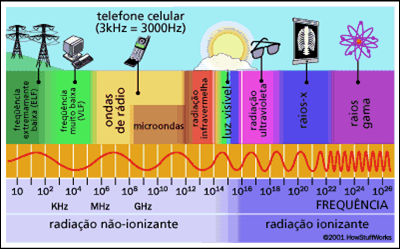
\includegraphics[width=0.75\textwidth]{./dados/figuras/figura_microondas}
    \caption{Comparação da radiação MO com as demais faixas de radiação eletromagnética}
    \fonte{\citeonline{trabalhoSeguro}}
    \label{fig:figura-mo}
\end{figure}

\section{MAGNETRON}
\label{sec:magnetron}

O magnetron consiste em um um tubo de vácuo de alta potência que gera radiação microondas através da interação de um fluxo de elétrons com um campo magnético. Os elétrons se movem entre uma série de cavidades de metal com aberturas chamadas de cavidades de ressonância. Um cátodo cilíndrico está no eixo principal, alguns milimetros distante de um ânodo circular. Dentro no ânodo, há diversas cavidades projetadas para ressonar em 2,45 GHz. Uma tensão da ordem de alguns kV é aplicada entre os eletrodos e um campo magnético é aplicado em paralelo ao eixo de forma que o campo elétrico e magnético fiquem perpendiculares entre si. Elétrons ejetados pelo cátodo aceleram radialmente no início devido ao campo elétrico mas começam a fazer trajetórias espirais devido a aceleração causada pelo campo magnético. Quando o campo magnético é forte demais, os elétrons não consegue chegar ao ânodo, e formam uma carga espacial giratória. As cavidades ressonantes do ânodo interagem com os elétrons, exercendo uma aceleração ou desaceleração. Finalmente, uma grande quantidade de elétrons oscila em volta do cátodo com frequências de microondas, que por sua vez gera oscilações auto-sustentáveis nas cavidades ressonantes, emitindo radiação microondas \cite{Vollmer}. A figura 2 mostra um diagrama do magnetron:

\begin{figure}[!htb]
    \centering
    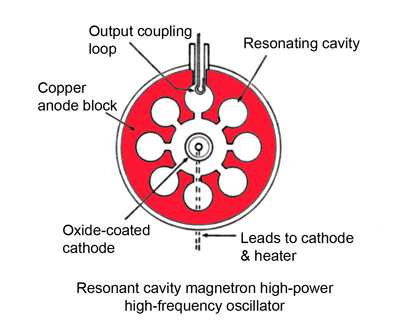
\includegraphics[width=0.75\textwidth]{./dados/figuras/magnetron}
    \caption{Diagrama de um Magnetron}
    \fonte{\citeonline{Vollmer}}
    \label{fig:figura-magnetron}
\end{figure}


\section{FONTES FERRO-RESSONANTES}
\label{sec:fontFerro}

Uma fonte ferro-ressonante é uma fonte baseada em transformador que usa características magnéticas não lineares e um circuito ressonante para providenciar uma tensão de saída estável sobre uma ampla faixa de tensões de entrada. Estas fontes são utilizadas em uma gama de aplicações que requerem tensões de saída constantes e especialmente utilizadas quando as tensões de entrada são instáveis devido à instabilidades das linhas de energia ou outros fatores, podendo absorver a maior parte dos transientes induzidos pela linha de transmissão. 

As fontes ferro-ressonantes são muito semelhantes a uma fonte incontrolável comum, exceto pelo fato da presença do transformador ferrorressonante, projetado especialmente para manter a tensão de saída constante em uma ampla faixa de tensões e correntes de entrada.  As principais desvantagens deste tipo de fonte são a sensibilidade a mudanças de frequência, a maior dissipação de calor em relação a transformadores comuns, a maior produção de ruído audível na ressonância e seu peso e tamanho em relação à fontes lineares \cite{PowerUk}. A figura 3 mostra um esquemático simplificado de uma fonte ferrorressonante, enquanto a figura 4 mostra uma fonte ferrorresonante em escala:


\begin{figure}[!htb]
    \centering
    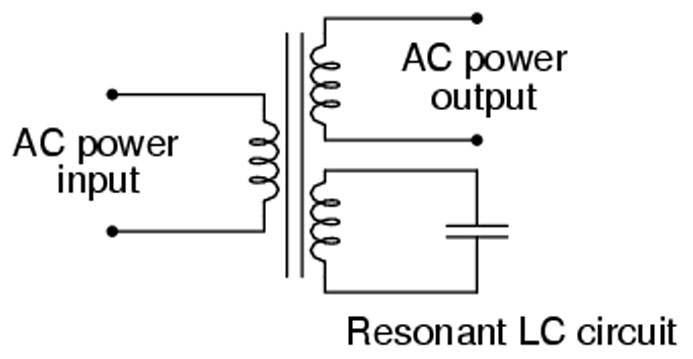
\includegraphics[width=0.6\textwidth]{./dados/figuras/font-ferro}
    \caption{Diagrama de uma fonte ferrorresonante}
    \fonte{\citeonline{PowerUk}}
    \label{fig:figura-fontferro}
\end{figure}

\pagebreak

\begin{figure}[!htb]
    \centering
    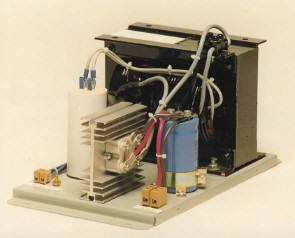
\includegraphics[width=0.4\textwidth]{./dados/figuras/font-ferro-real}
    \caption{Fonte ferrorresonante em escala}
    \fonte{\citeonline{PowerUk}}
    \label{fig:figura-fontferro}
\end{figure}



\section{FUNCIONAMENTO DO FORNO MICROONDAS}
\label{sec:funcMicro}

O forno microondas consiste em duas partes principais: o magnetron, o qual é alimentado por uma fonte com uma grande tensão de saída, e a câmara de cozimento, que é revestida por paredes metálicas e contém uma plataforma giratória para rotacionar o alimento. A medida que o magnetron gera radiação, as ondas eletromagnéticas chegam à câmara através de um guia de onda acoplado ao magnetron. Este guia geralmente é uma seção retangular de um tubo metálico. Uma vez que as MO chegam à câmara, elas são efetivamente refletidas pelas paredes metálicas. As ondas ressonam na cavidade e formam ondas estacionárias. Devido à frequência das ondas, cerca de 2,45 GHz, o comprimento de onda é da ordem das dimensões lineares da câmara. A figura abaixo mostra um diagrama de funcionamento de um forno convencional:

\begin{figure}[!htb]
    \centering
    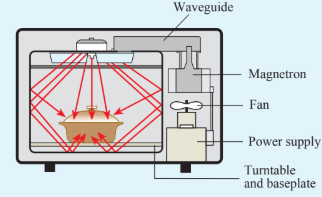
\includegraphics[width=0.6\textwidth]{./dados/figuras/microwave}
    \caption{Diagrama de funcionamento um forno microondas convencional}
    \fonte{\citeonline{Vollmer}}
    \label{fig:figura-fontferro}
\end{figure}

Num forno ideal, toda o alimento seria cozido de forma uniforme, porém, na prática os nós das ondas estacionárias geradas fazem que o alimento aqueça e algumas partes e permaneça frio em outras. A figura 6 mostra a distribuição de temperatura dentro de um forno microondas de dimensões  29 x 29 x 19 cm³, em um altura de cerca de 8 cm acima do fundo da cavidade. Um prato de vidro horizontal  com uma fina camada de água foi colocado 15 s em um microondas sem a plataforma giratória em potência máxima (cerca de 800 W). Com uma pequena quantidade de água presente, a imagem mostra o padrão de intensidade em uma câmara quase vazia. Nota-se uma existência pronunciada de modos de ressonância horizontais, o que geraria um aquecimento não uniforme. Esta não uniformidade é a principal razão para a existência da plataforma giratória, que levaria o alimento a diferentes nós quentes e frios \cite{Vollmer}. No entanto, mesmo com a plataforma o alimento ainda é cozido de forma não uniforme, devido à complexa interação entre as MO e os alimentos e as diferentes interações que cada parte do alimento tem com cada um dos nós e antinós.

\begin{figure}[!htb]
    \centering
    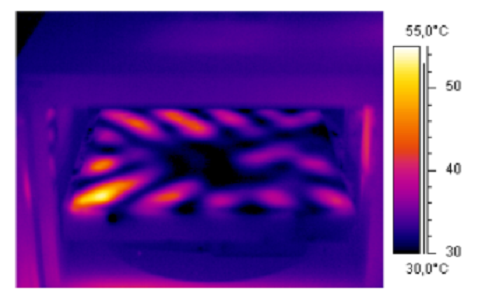
\includegraphics[width=0.6\textwidth]{./dados/figuras/micronodes}
    \caption{Visualização da estrutura dos modos de propagação horizontais em um forno microondas utilizando imagens termais infravermelhas. Um prato de vidro com uma fina camada de água foi colocado de uma altura de 8 cm e aquecido por 15 s em uma potência de 800 W.}
    \fonte{\citeonline{Vollmer}}
    \label{fig:figura-fontferro}
\end{figure}


\section{INVERSORES RESSONANTES}
\label{sec:inverter}

Inversores ressonantes são um tipo de inversor baseados em oscilações ressonantes de corrente.  Inversores ressonantes série são colocados em série com a carga para formar um circuito sub-amortecido. A corrente através destes dispositivos de chaveamento chega a zero devido a natureza do circuito. Se o dispositivo for um tiristor, diz-se que o dispositivo é auto-comutado. 
Este tipo de inversor produz uma forma onda aproximadamente senoidal de frequências que podem variar de 20 kHz até 100 MHz e é comumente usados em aplicações que necessitam de tensão constante, como lâmpadas fluorescentes, geradores ultra sônicos ou aquecimento por indução. Devido a alta frequência de chaveamento, os componentes do inversor ressonantes tem tamanho reduzido \cite{Rashid}.

\begin{figure}[!htb]
    \centering
    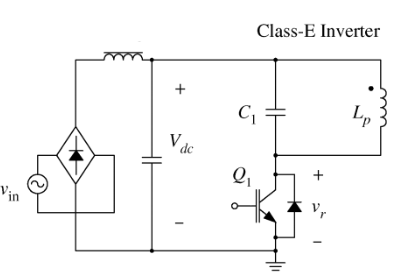
\includegraphics[width=0.6\textwidth]{./dados/figuras/inverter}
    \caption{Inversor ressonante classe E}
    \fonte{\citeonline{Woo}}
    \label{fig:figura-fontferro}
\end{figure}


\section{MICROCONTROLADORES}
\label{sec:micro}

Um microcontrolador, ou UC (acrônimo para   $\mu$-controlador) é um pequeno computador em um único circuito integrado. Um microcontrolador pode ter uma ou mais CPUs, isto é núcleos de processamento, juntamente com uma memória e periféricos de entrada e saída programáveis. Memória na forma de \textit{flash} ou ROM é inclusa no \textit{chip}, em conjunto com uma pequena quantidade de memória RAM. Microcontroladores são projetados para aplicações embarcadas, em contraste com os microprocessadores utilizados nos computadores pessoais. Geralmente os UC são aplicados em produtos ou dispositivos controlados automaticamente, tais como sistemas de controle para motores ou controles remotos. Por terem tamanhos e custo reduzidos em relação a um projeto que utiliza um microprocessador, memória e dispositivos de I/O separadamente, os UC são economicamente vantajosos para fazer o controle de um dispositivo ou processo.


\begin{figure}[!htb]
    \centering
    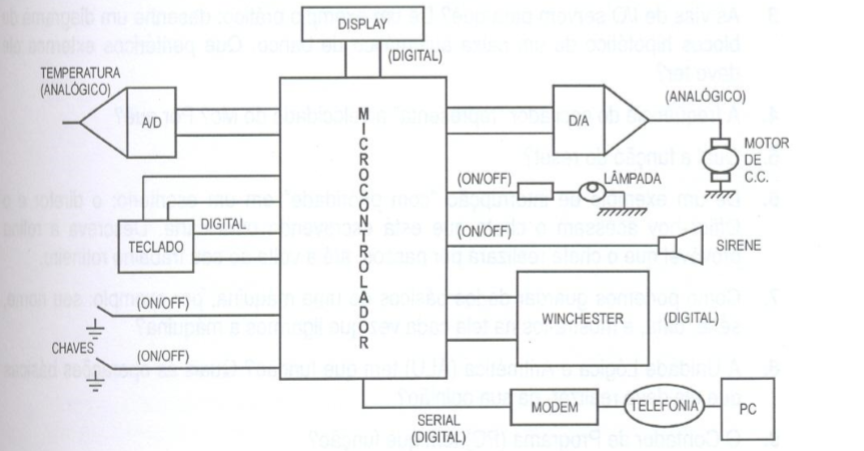
\includegraphics[width=0.9\textwidth]{./dados/figuras/micro}
    \caption{Ilustração hipotética de um microcontrolador e seus periféricos}
    \fonte{\citeonline{Nicolosi}}
    \label{fig:figura-uc}
\end{figure}

\pagebreak 

\section{USO DE IGBTS EM PARALELO}
\label{sec:paralleligbt}

Em muitas aplicações, em vez de se empregar um IGBT projetado para atuar em determinada faixa de tensão, pode-se utilizar dois IGBTs menores conectados em paralelo. As vantagens deste tipo de conexão são um uma organização mais flexível e individual do \texit{layout}, fazendo com que as fontes de calor estejam mais distribuídas, de modo que maiores níveis de perdas sejam mitigados. No entanto, a principal desvantagem é a divisão desigual das perdas. A principal razão para isto é a variabilidade entre os parâmetros dos dois dispositivos, os quais dependem muito do fabricante. Outro motivo que pode levar a diferença citada é o uso de circuitos de alimentação assimétricos \cite{Infineon}.
            
\begin{figure}[!htb]
    \centering
    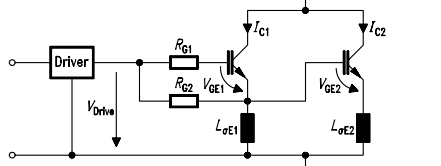
\includegraphics[width=0.9\textwidth]{./dados/figuras/paralleligbt}
    \caption{Esquemático de uso de IGBTs em paralelo}
    \fonte{\citeonline{Infineon}}
    \label{fig:figura-paralleligbt}
\end{figure}

\section{CONTROLADOR PROPORCIONAL INTEGRAL}
\label{sec:pi-controller}
O controlador Proporcional Integral (PI) é um mecanismo de controle em malha fechada empregando realimentação. Este controlador cálcula constantemente constantemente o erro variante no tempo que é a diferença entre o \textit{set-point} e o valor da variável de processo medida. A figura abaixo mostra uma representação da malha de controle PI, com a fórmula do algorítmo:

\begin{figure}[H]
    \centering
    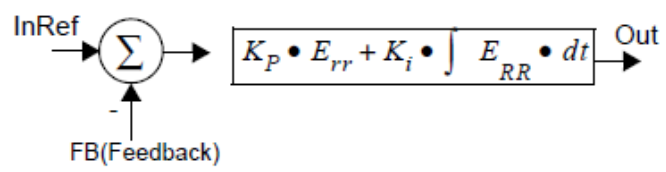
\includegraphics[width=0.9\textwidth]{./dados/figuras/pi-controller}
    \caption{Controlador PI}
    \fonte{\citeonline{Apmonitor}}
    \label{fig:figura-pi-controller}
\end{figure}

Os dois valores de ajuste para o controlador PI são as constantes proporcional e integrativa. A constante proporcional é o que se chama de ganho do controlador, que irá apenas multiplicar a diferença entre o \textit{set point} e o valor da variável de processo medida. Já a constante integrativa é um multiplicador do erro proporcional, e um valor maior torna o controlador mais agressivo, de modo a diminuir o tempo de resposta ao passo que aumenta a instabilidade.

%%\null
%%\vfill         % Revisão de Literatura
% METODOLOGIA------------------------------------------------------------------
\chapter{PROCEDIMENTOS METODOLÓGICOS}
\label{chap:metodologia}

Este capítulo tem como finalidade descrever a metodologia e os procedimentos adotados na confecção deste projeto, bem como também realizar uma consolidação de todos os métodos aqui utilizados e apresentar o funcionamento do sistema como um todo. Para tal, os procedimentos metodológicos foram divididos da seguinte forma: Fonte inversora (Seção 3.1),  \textit{Shunt} (Seção 3.2), DSPIC33  (Seção 3.3), Circuito de controle (Seção 3.4), Planta (Seção 3.5)

\section{FONTE INVERSORA}
\label{sec:fonteInversora}

Para realizar a alimentação do magnetron, foi utlizada uma fonte inversora, a qual consiste em um inversor ressonanete classe E. Segundo \citeonline{Hidenori1991}, uma fonte inversora tem as seguintes vantagens em relação à uma fonte ferrorressonante tradicional:
\begin{itemize}
    \item Potência de saída controlável;
    \item Maior eficiência energética;
    \item Circuito menor e mais leve;
    \item Pode operar em maior frequência.
\end{itemize} 

\begin{figure}[!htb]
    \centering
    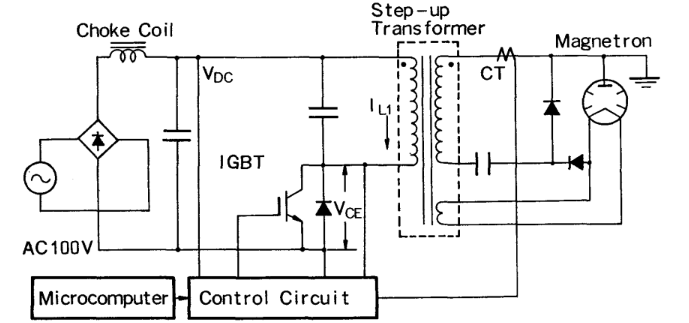
\includegraphics[width=0.9\textwidth]{./dados/figuras/font_inverter}
    \caption{Fonte inversora para alimentação do magnetron}
    \fonte{\citeonline{Hidenori1991}}
    \label{fig:figura-inverter}
\end{figure}

\subsection{Simulações}
\label{sec:simulations}

Para verificar se a fonte inversora é viável para o projeto, foram feitas simulações do circuito no software \textit{PSIM}. Na alimentação o magnetron, são necessários cerca de 4 kV. Assim, primeiramente foi desenvolvido um circuito para simular a alimentação de uma carga de cerca de 100 M$\Omega$, com uma tensão de entrada de 127 V. A figura a seguir mostra o circuito desenvolvido:

\begin{figure}[!htb]
    \centering
    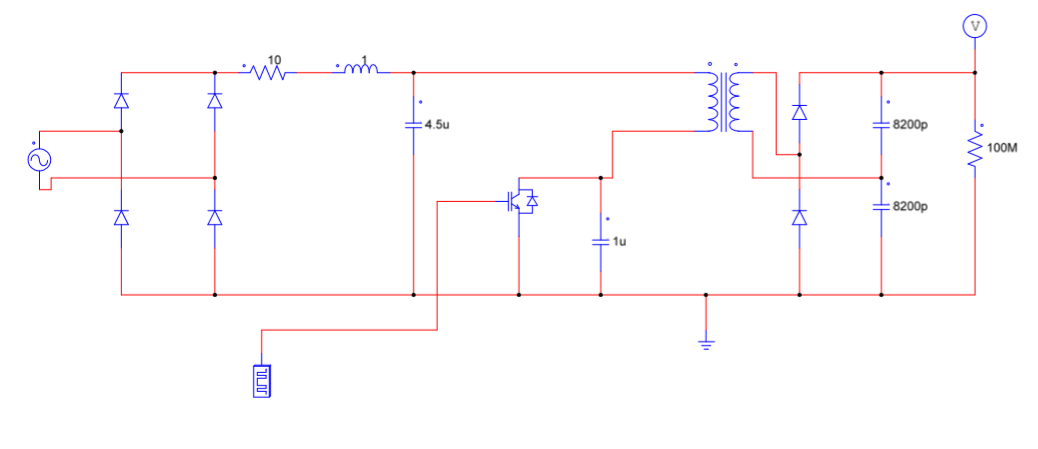
\includegraphics[width=0.9\textwidth]{./dados/figuras/psim1}
    \caption{Circuito da fonte inversora simulada}
    \fonte{Autoria própria (2019)}
    \label{fig:circ_sim_1}
\end{figure}

Para averiguar se uma fonte inversora consegue alimentar uma carga de alta potência à uma tensão de alguns kV, o inversor foi chaveado em um ciclo de trabalho de 50\%. A figura abaixo mostra a froma de onda da tensão na carga resistiva:

\begin{figure}[!htb]
    \centering
    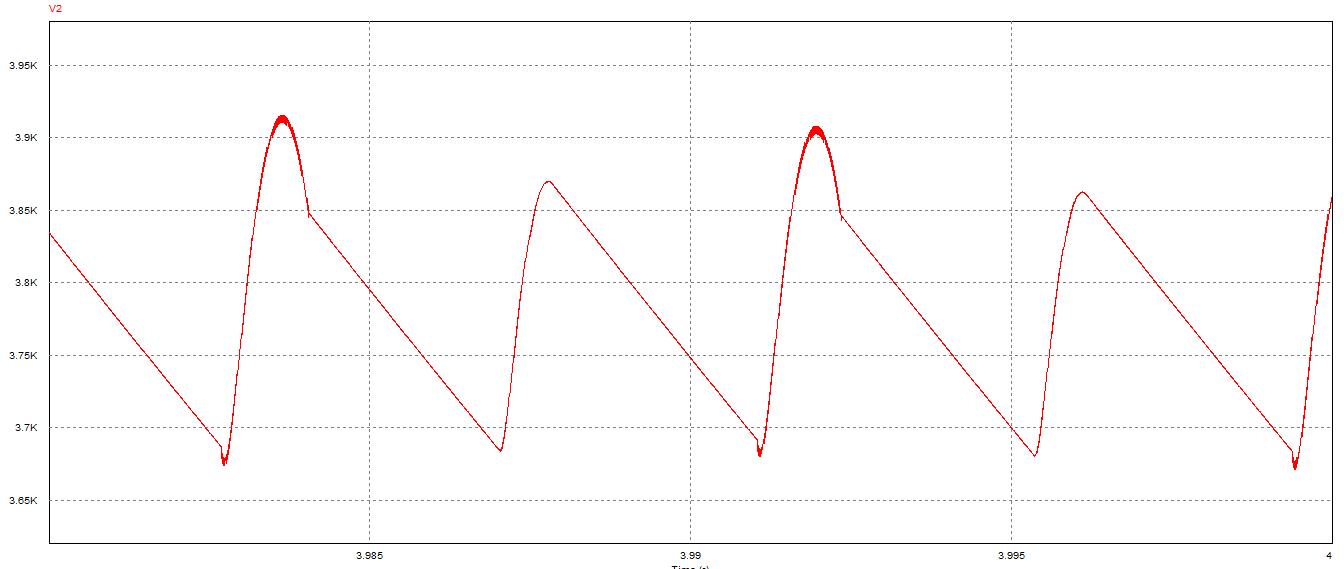
\includegraphics[width=0.9\textwidth]{./dados/figuras/psim2}
    \caption{Forma da onda simulada da tensão na carga}
    \fonte{Autoria própria (2019)}
    \label{fig:figura-graf_sim_1}
\end{figure}

Na figura \ref{fig:figura-graf_sim_1}, pode-se ver que o pico de tensão da carga chega à quase 4 kV, o que já é suficiente para o objetivo em questão. Logo, conclui-se que a fonte inversora é viável para a alimentação do circuito de um magnetron.

\subsection{Projeto}

O projeto da fonte inversora se baseou em boa parte no conceito desenvolvido por \citeonline{Hidenori1991}. O chaveamento do circuito é feito por um microcontrolador que é realimentado por um sensor de corrente. Foram utilizados IGBTs em paralelo para aumentar a potência dos sistemas e reduzir perdas no dispositivo. Um transformador de três fios de alta potência alimenta as entradas que são ligadas ao magnetron com alta tensão. A tensão de entrada do circuito é a tensão da rede retificada por uma ponte de diodos. O circuito foi desenvolvido no software \texit{Altium Desginer}. A figura \ref{fig:proj-font-inv} mostra o circuito projetado:

\begin{figure}[!htb]
    \centering
    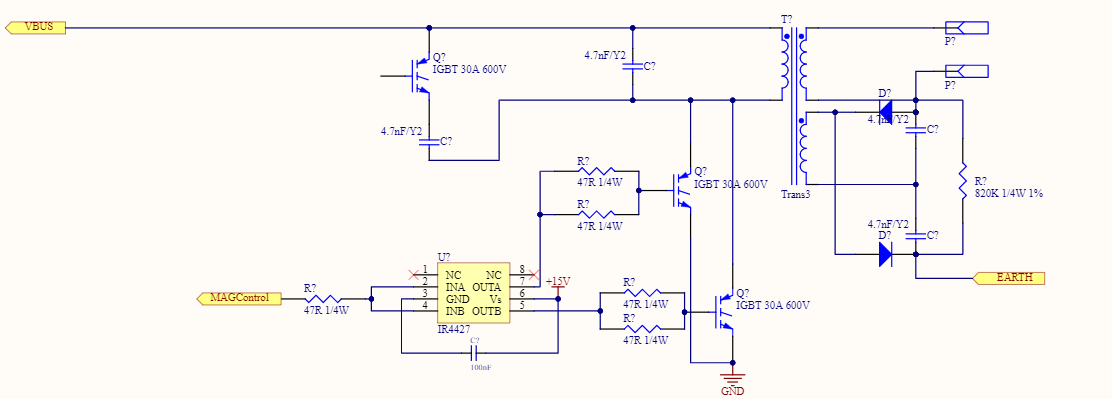
\includegraphics[width=1.1\textwidth]{./dados/figuras/proj-font-inv}
    \caption{Circuito projetado}
    \fonte{Autoria própria (2019)}
    \label{fig:proj-font-inv}
\end{figure}

\subsection{Descrição de funcionamento}

\subsection{Montagem}

\section{\texit{Shunt}}
\label{sec:shunt}


\section{DSPIC33}
\label{sec:dsPIC}

O DSPIC33 é um microntrolador da família PIC, desenvolvido pela Microchip Technology Inc., que possui funcionalidade de processador digital de sinais (DSP). Este componente foi escolhido para fazer o controle do chaveamento da fonte inversora pois consegue operar em uma ampla faixa de temperatura e possui diversas funcionalidades interessantes para o controle de sinais analógicos de alta frequência. Algumas das funcionalidades, cruciais para o projeto, incluem:

\begin{itemize}
    \item Módulo ADC configurável de 10 bits e amostragem de 1.1 Msps ou 12 bits e amostragem de 500 ksps;
    \item Três amplificadores operacionais integrados ao ADC da plataforma;
    \item Interrupções de \textit{Change Notification} em todos os pinos de I/O;
    \item \textit{Timers} e contadores de 32 bits;
    \item Funções de PWM de alta velocidade.
\end{itemize} 

\begin{figure}[!htb]
    \centering
    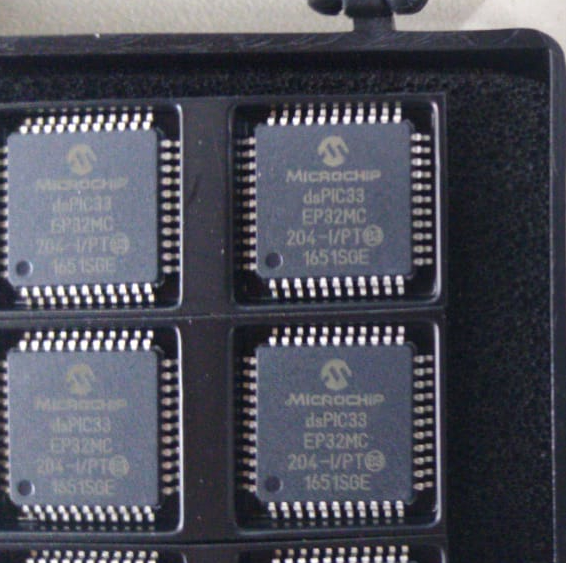
\includegraphics[width=0.3\textwidth]{./dados/figuras/dspic}
    \caption{Microcontrolador DSPIC33}
    \fonte{Autoria própria (2019)}
    \label{fig:figura-dspic}
\end{figure}

A CPU da plataforma possui arquitetura Harvard, típica da família de processadores PIC, possuindo uma palavra de instrução de 24 bits e 12 MB de endereços de memória de programa. O microprocessador possui um extenso suporte ao processamento digital de sinais, tendo acumuladores e ULA de 40 bits, dois multiplicadores de alta velocidade 17 por 17 bits e um \textit{barrell shifter} de 40 bits que consegue alternar 16 bits em úniclo ciclo de \textit{clock}. A arquitetura do processador fornece uma compilação eficiente de código, suportando a linguagem C e \textit{Assembly}.

No circuito, o microcontrolador...

\begin{figure}[!htb]
    \centering
    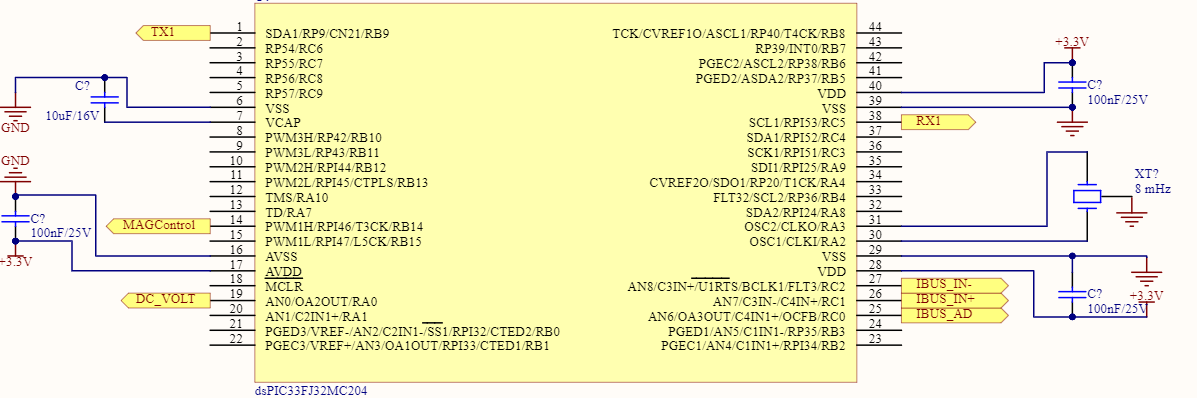
\includegraphics[width=0.9\textwidth]{./dados/figuras/proj-uc}
    \caption{Esquemático do microcontrolador no circuito}
    \fonte{Autoria própria (2019)}
    \label{fig:figura-dspic}
\end{figure}


\section{CIRCUITO DE CONTROLE}
\label{sec:controlCircuit}



\section{PLANTA}
\label{sec:plant}

                   % Metodologia
%% RESULTADOS-------------------------------------------------------------------

\chapter{APRESENTAÇÃO E ANÁLISE DE RESULTADOS}

Aqui serão detalhados os resultados obtidos com o funcionamento do circuito desenvolvido integrado a um forno microondas convencional da marca Panasonic. Nesta capítulo será descrito o funcionamento prático do circuito, expondo o resultado da medições de parâmetros que avaliam a performance e fazendo comparações com os parâmetros do circuito ferrorressonante, os quais estão disponíveis na literatura. 


\section{Sistema em Funcionamento}
A placa original do aparelho foi removida e trocada pela placa desenvolvida, ligando-se todos os fios que conectam o circuito projetado à rede e ao magnetron maneira similar à original. Para acionar o circuito, foi utilizada a interface já presente no forno, configurando o nível percentual de potência e o tempo de cozimento de acordo com os experimentos realizados. Para testar o funcionamento, a equipe acionou o circuito em diferentes configurações de potência, medindo-se as formas de onda em diferentes pontos para demonstrar o funcionamento prático do sistema. As subseções a seguir irão descrever este funcionamento.

\subsection{Corrente e potência}
A fim de se verificar o funcionamento correto do circuito montado, as formas da corrente no \textit{shunt} foram verificadas com um osciloscópio digital. A figura abaixo mostra o resultado obtido com o circuito operando em potência máxima:

\begin{figure}[H]
    \centering
    \caption{Formas de onda da tensão e corrente}
    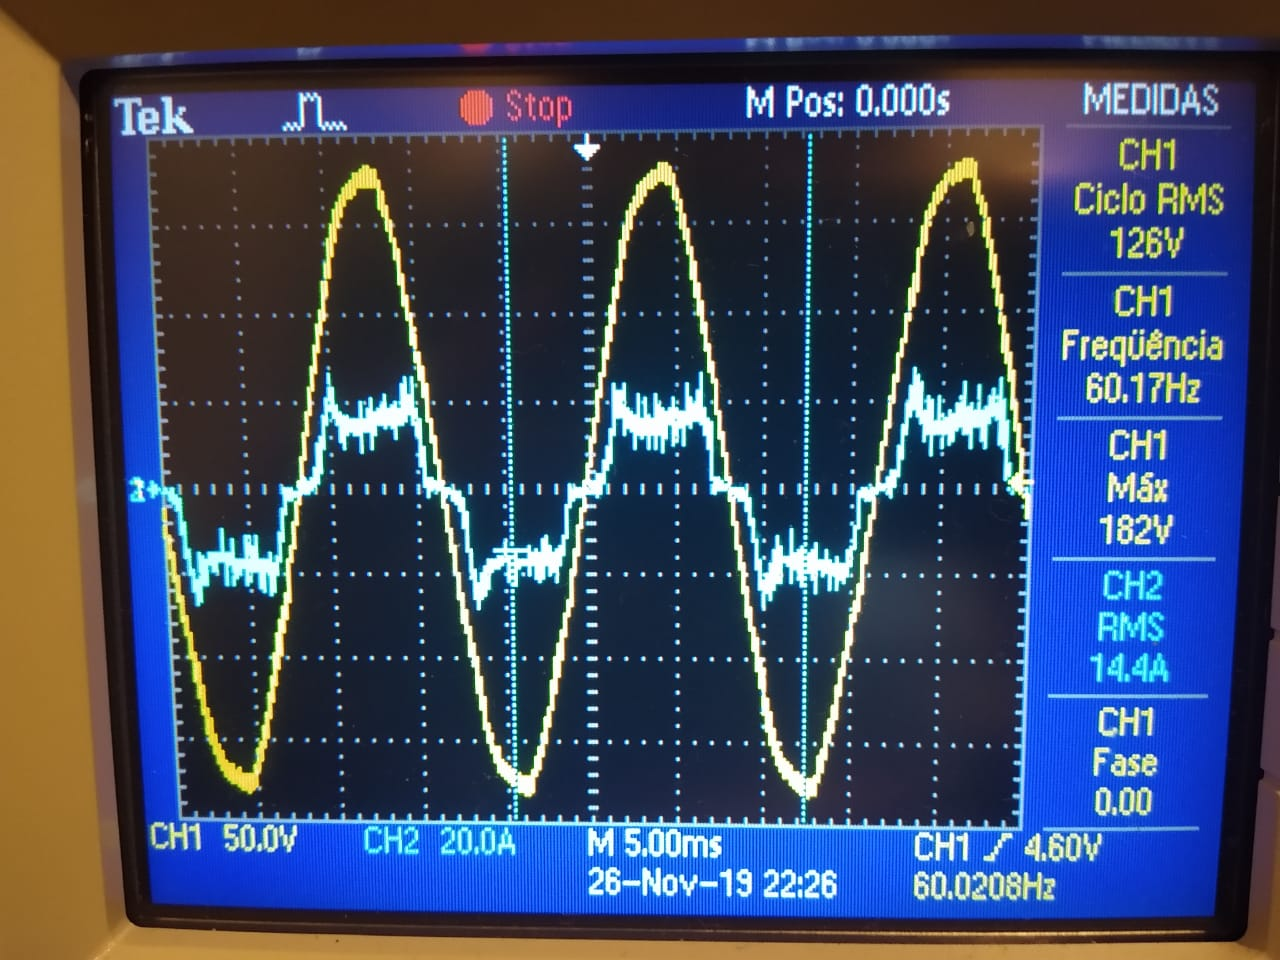
\includegraphics[width=0.8\textwidth]{./dados/figuras/onda_corrente}
    \fonte{Autoria própria (2019)}
    \label{fig:figura-onda_corrente}
\end{figure}

Na figura, a forma de onda azul (canal 2) é a corrente no \textit{shunt}, enquanto a outra forma de onda, em amarelo (canal 1) é a tensão da rede. Como pode-se observar, o valor da corrente é muito elevado, atingindo um valor RMS de 14,4 A.  A medida que o nível de potência varia, maior o valor RMS da corrente e mais a forma de onda tende a suavizar a curvatura que tem em direção ao eixo horizontal. A forma de onda segue o mesmo ciclo que o sinal da tensão da rede, tendo um \textit{ripple} extremamente elevado. Este \textit{ripple} nada mais é que a consequência do forte ruído gerado pelas emissões do magnetron. Saleinta-se que o ambiente do experimento não era controlado, e que o chassi metálico do forno não estava fechado, o que contribui também para distorções na forma de onda.

Para medir a potência consumida pelo circuito, foi utilizado um medidor de energia elétrica comercial portátil, no qual se conecta a alimentação do forno, enquanto a alimentação do medidor é ligada na tomada no lugar do aparelho. A figura abaixo mostra a leitura obtida no mesmo experimento:

\begin{figure}[H]
    \centering
    \caption{Leitura de potência obtida}
    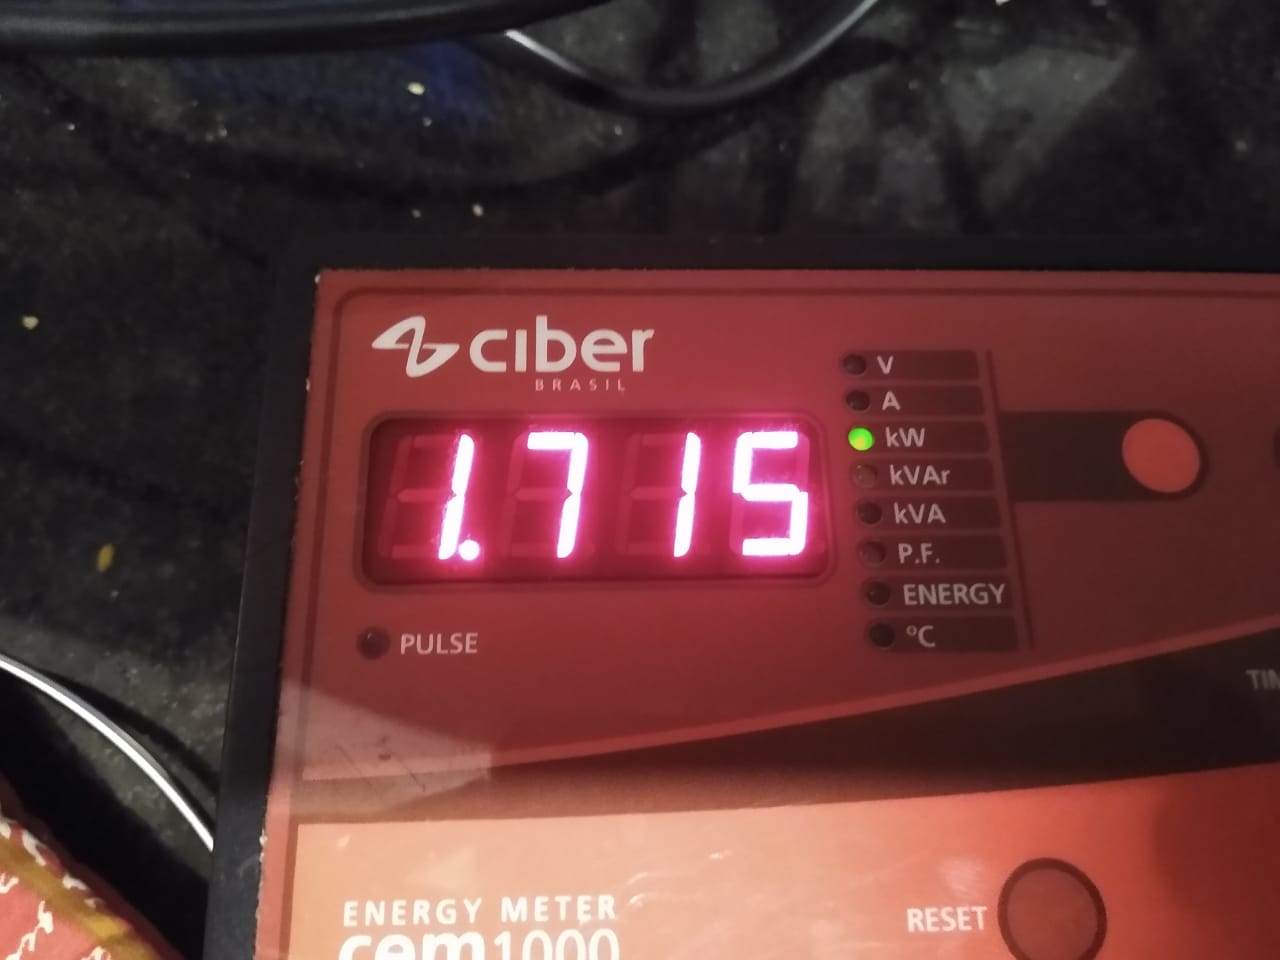
\includegraphics[width=0.8\textwidth]{./dados/figuras/medida_potencia_full}
    \fonte{Autoria própria (2019)}
    \label{fig:figura-medida_potencia_full}
\end{figure}

A leitura obtida, como pode-se notar, é de 1715 W. Ao calcular-se a potência teórica pelos valores RMS medidos na figura \ref{fig:figura-onda_corrente}, obtém-se 1814 W. Para este experimento não foi feita uma calibração com os devidos equipamentos, e portanto não se tem uma precisão elevada para as medições. Outro fator que influencia na precisão, é o elevado ruído de alta frequência detectado na forma de onda da corrente, que também deteriora a qualidade da medição. Para este experimento, a equipe configurou o algoritmo de controle com uma potência máxima de 1700 W. Devido aos fatores prejudiciais à precisão do experimento, citados anteriormente, o valor real da potência atingida pode sofrer uma pequena alteração percentual. De forma geral, tem-se que a potência obtida pelo experimento está dentro do que foi esperado pela equipe, visto que em ambas as medições o valor medido não ultrapassou os 10\% de tolerância estabelecido pela equipe.

\subsection{Chaveamento dos IGBTs}
O chaveamento dos IGBTs é o que faz efetivamente o controle da potência do magnetron, bloqueando o sinal de tensão no primário quando os dispositivos são colocados em \textit{off}. Para realizar o controle, a planta desenvolvida controla dois parâmetros do sinal da porta do dispositivo: frequência e ciclo de trabalho. As figuras abaixo mostram o circuito operando em três configurações. Em amarelo, no canal 1 é mostrado o sinal do IGBT. Em azul, no canal 2, é mostrada a tensão de barramento, enquanto no canal 3, em rosa, mostra-se o sinal que vai para o conversor AD de tensão:

\begin{figure}[H]
    \centering
    \caption{Formas de onda: caso 1}
    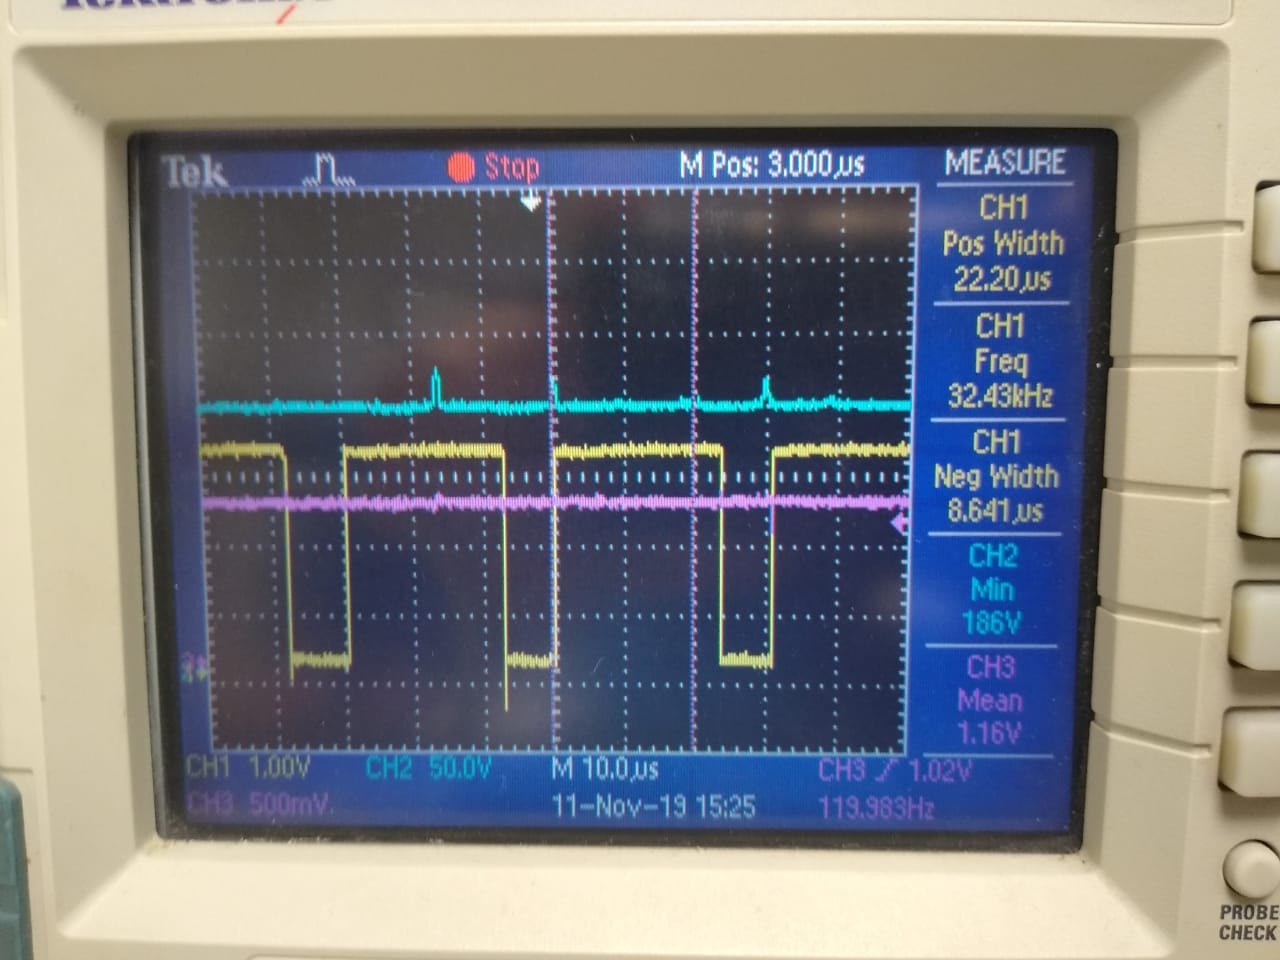
\includegraphics[width=0.8\textwidth]{./dados/figuras/onda_controller_1}
    \fonte{Autoria própria (2019)}
    \label{fig:figura-onda_controller_1}
\end{figure}

\begin{figure}[H]
    \centering
    \caption{Formas de onda: caso 2}
    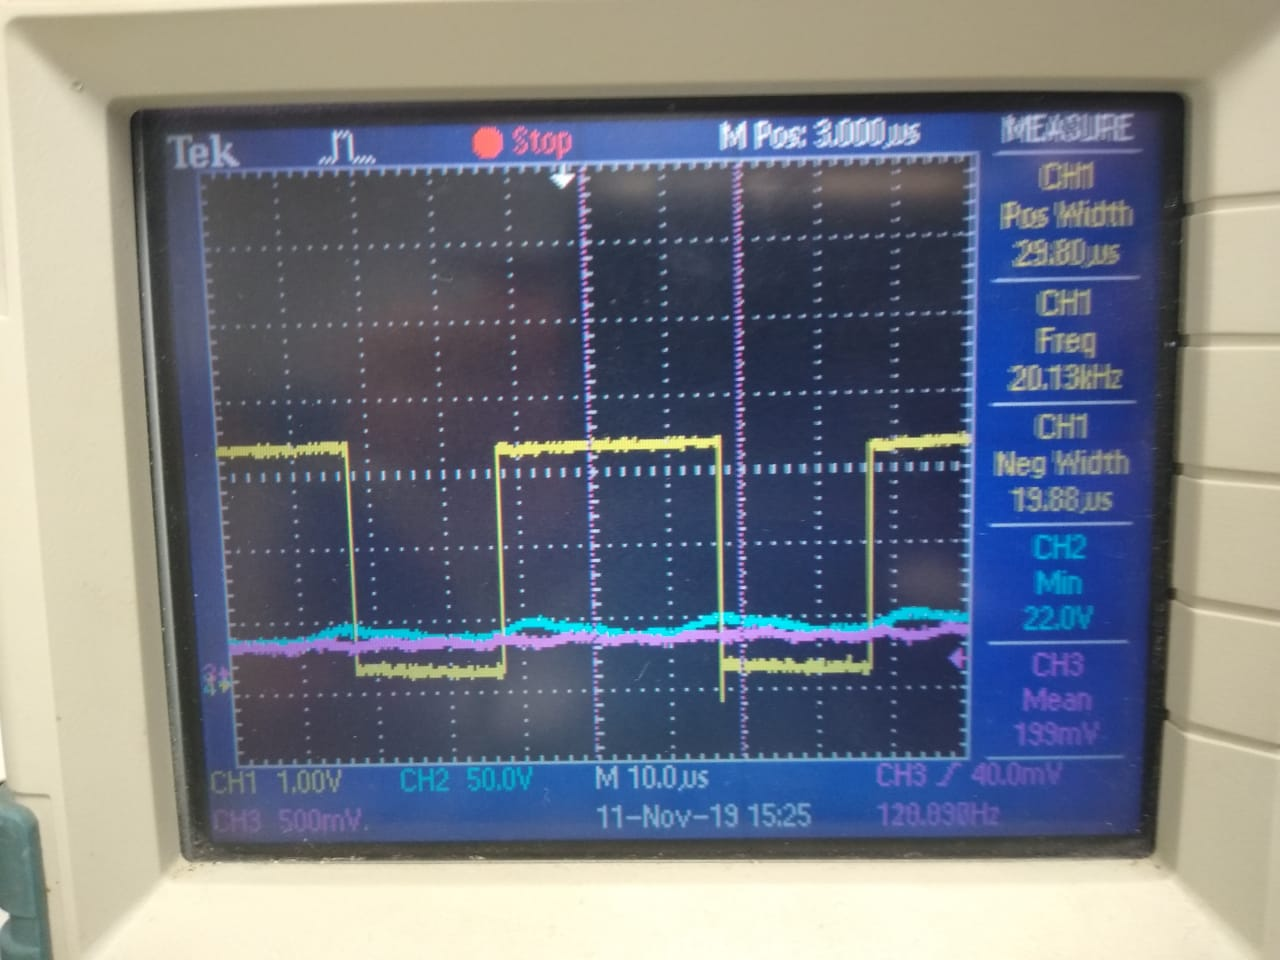
\includegraphics[width=0.8\textwidth]{./dados/figuras/onda_controller_2}
    \fonte{Autoria própria (2019)}
    \label{fig:figura-onda_controller_2}
\end{figure}

\begin{figure}[H]
    \centering
    \caption{Formas de onda: caso 3}
    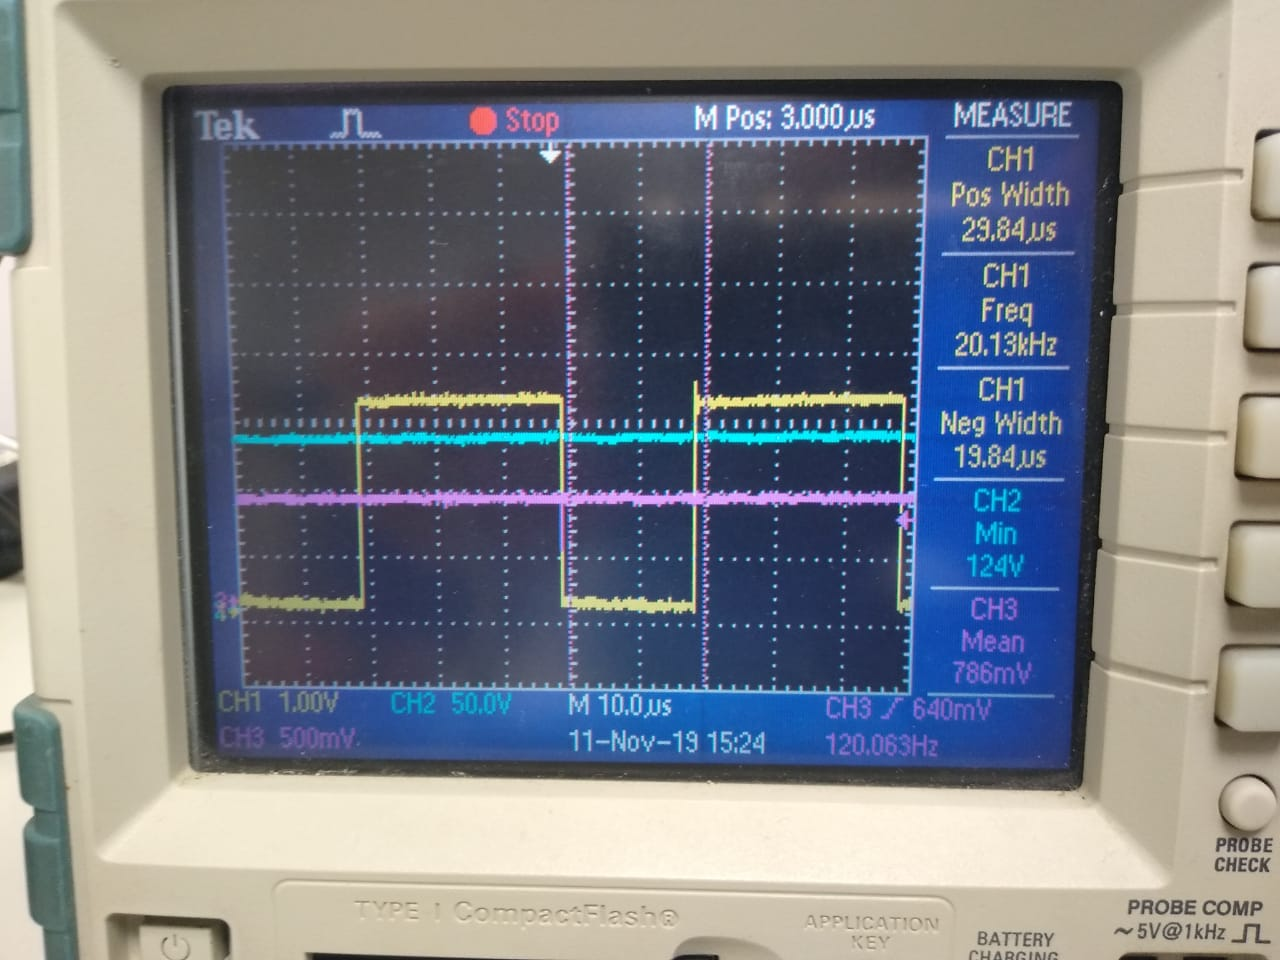
\includegraphics[width=0.8\textwidth]{./dados/figuras/onda_controller_3}
    \fonte{Autoria própria (2019)}
    \label{fig:figura-onda_controller_3}
\end{figure}

Nas figuras mostradas, tem-se três situações: 
\bigskip
\begin{itemize}
    \item Ciclo de trabalho 70\%, frequência de 32 kHz e tensão do ADC de 1,16 V;
    \item Ciclo de trabalho 60\%, frequência de 20 kHz e tensão do ADC de 199 mV;
    \item Ciclo de trabalho 60\%, frequência de 20 kHz e tensão do ADC de 786 mV.
\end{itemize}
\bigskip

Cada situação mostra uma diferente decisão tomada pelo \textit{firmware} desenvolvido. A planta desenvolvida, através da realimentação de \textit{corrente} e cálculo da potência com a medição do conversor AD, determinou o valor do ciclo e trabalho e frequência utilizada no chaveamento para regular a potência no valor estabelecido. Um maior ciclo de trabalho não implica necessariamente numa maior potência, visto que a frequência do sinal exerce um papel fundamental na determinação da potência de saída, dadas às características do circuito.

\subsection{Sinais de controle e status}
Os sinal de controle determina a potência solicitada pelo magnetron e o sinal de status verifica se o sistema está operando corretamente. A figura abaixo mostra as formas de onda medidas destes dois sinais operando com potência máxima:

\begin{figure}[H]
    \centering
    \caption{Formas de onda dos sinais de comunicação}
    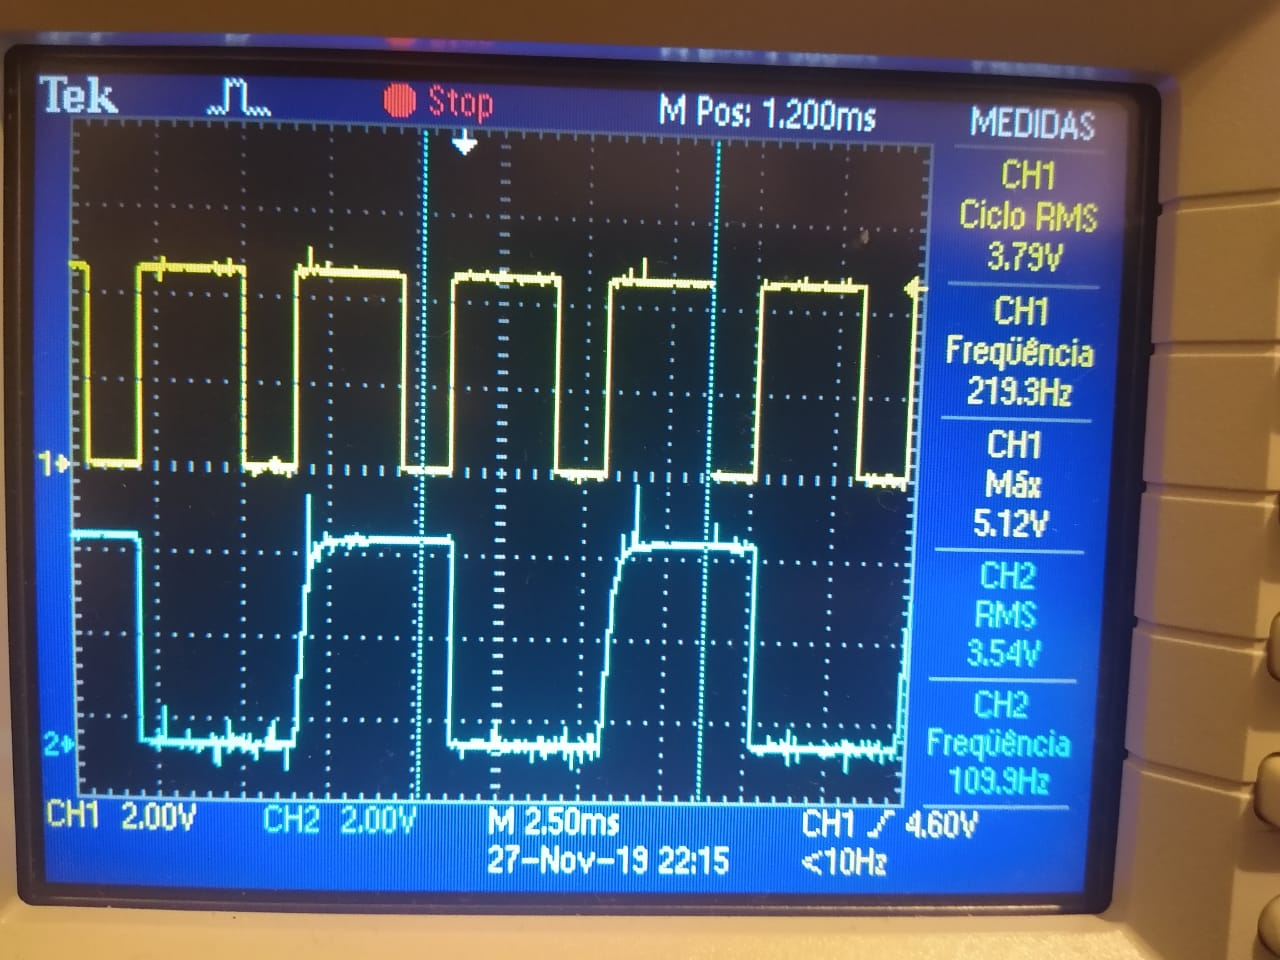
\includegraphics[width=0.8\textwidth]{./dados/figuras/onda_comm}
    \fonte{Autoria própria (2019)}
    \label{fig:figura-onda_comm}
\end{figure}

Em amarelo, no canal 1, é mostrado o sinal de controle. O ciclo de trabalho de 75\% representa a solicitação de potência máxima. Caso a potência solicitada diminua, o ciclo de trabalho também irá diminuir, e abaixo de um ciclo de 50\%, a forma de onda deixa de ser continua, ficando um determinado intervalo de tempo com 0 V. Quanto ao sinal de status, nota-se que o mesmo é uma onda quadrada contínua, com ciclo de trabalho fixado em 50\%, sendo sincronizado com a forma de onda do sinal de controle. Portanto, de acordo com o projeto do algoritmo para a interface de comunicação, descrito na seção \ref{sec:plant}, pode-se considerar que o resultado obtido está de acordo com o comportamento previsto.


\section{Medições de parâmetros}
Para comparar o desempenho do circuito desenvolvido com uma fonte ferrorressonante tradicional, foram medidos três parâmetros essenciais para se possibilitar uma discussão válida sobre o tema: eficiência, fator de potência e dimensões físicas, incluindo massa, altura, largura e comprimento. 

\subsection{Eficiência}
A eficiência do forno microondas pode ser avaliada de forma geral como a performance do circuito de alimentação do magnetron. Este parâmetro pode ser obtido fazendo-se uma relação entre o calor absorvido pelo líquido dentro na câmara de cozimento do forno e a energia elétrica consumida pelo circuito.
Para avaliar a performance, a equipe se baseou em um experimento que é utilizado pelo INMETRO para determinar a eficiência de fornos microondas, o qual está detalhado em \cite{Inmetro}. O experimento consiste em esquentar 1 litro de água em um determinado tempo. A realização do experimento não seguiu totalmente os critérios estipulados pelo INMETRO, visto que a experiência não foi feita em ambiente controlado e o recipiente utilizado não é possui as dimensões, peso e material recomendados. A água usada no teste estava armazenada em um recipiente aberto de vidro, o qual tem massa de 600g. Antes da realização da experiência, a equipe aqueceu o recipiente vazio para determinar se o mesmo aquecia de forma significativa sem a presença de água, a fim de verificar se o recipiente poderia interferir nas medições. Inicialmente o recipiente se encontrava em temperatura ambiente de 20 ºC. Após colocá-lo no microondas por 60 segundos, o recipiente apresentou temperatura de 22 ºC. Logo a variação foi de 2 ºC, a qual não acarreta em impactos significativos na precisão das medidas.
Inicialmente mediu-se a temperatura da água no recipiente, utilizando-se um termopar industrial comum. Feito isso, o recipiente foi colocado no forno e acionado em potência máxima durante 65 segundos. Então, retirou-se a o recipiente do aparelho e com o termopar mediu-se a temperatura. Através das fórmulas descritas em cite, mediu-se a eficiência do circuito. No total, foram realizados dois experimentos, cada qual possuindo uma temperatura da água distinta. O tempo de aquecimento não é o tempo de cozimento selecionado no teclado do forno pois o magnetron utilizado leva cerca de 4 segundos para ter seu filamento aquecido e começar a emitir radiação. Seja $T_i$ a temperatura inicial, $T_f$ a temperatura final, $T_\mathrm{amb}$ a temperatura ambiente, $t_\mathrm{total}$ o tempo de cozimento configurado, $t_\mathrm{aq}$  o tempo de aquecimento do filamento,  $W_\mathrm{in}$ a energia consumida durante o ensaio, $P$ a potência de saída de microondas calculada, e $\eta$ a eficiência energética. A tabela abaixo mostra os resultados obtidos em todas as leituras:
\begin{table}[H]
    \centering
    \caption{Resultados obtidos nos ensaios}
    \begin{tabular}{|l|l|l|l|l|l|l|l|l|} 
	\hline
	$T_i$ (ºC) &$T_f$ (ºC)	&$T_\mathrm{amb}$ (ºC)	 &$t_\mathrm{total}$ (s)	&$t_\mathrm{aq}$ (s)	 &$t_\mathrm{total}$  -  $t_\mathrm{aq}$	&$P$ (W)	&$W_\mathrm{in}$ (Wh)	&$\eta$ (\%)\\\hline	
	18	&7	&19	&65	&4	&61	&749,623	&28	&45,36\\\hline	
	33	&22	&20	&75	&4	&71	&709,113	&31	&45,11\\\hline
    \end{tabular}
    \label{table-eff}
\end{table}


Da tabela \ref{table-eff}, percebe-se que o valor da eficiência obtida pelos experimentos é muito próximo. Isto demonstra que o circuito possui um comportamento regular, apresentando pouca variação conforme o aumento de temperatura da água. Este comportamento é relevante pois mostra que o calor transmitido mantém-se constante em determinada faixa de temperatura, sugerindo que a uniformidade do aquecimento tende a se manter a mesma ao passo que a temperatura aumenta. Conforme a edição de 2016 do programa brasileiro de etiquetagem e com os resultados medidos, o circuito desenvolvido se encaixaria na categoria C de eficiência energética, com eficiência de 45\% \cite{Etiquetagem}.

\subsection{Fator de Potência}

Na medição o fator de potência,  utilizou-se o mesmo dispositivo usado para medir a potência mostrado na figura k. O circuito foi ligado em diversas configurações de potência, medindo-se o fator de potência com o mesmo dispositivo usando na figura \ref{fig:figura-medida_potencia_full} de cada configuração em um minuto de aquecimento. A tabela abaixo contém os resultados obtidos:

\begin{table}[H]
    \centering
    \caption{Resultados de fator de potência obtidos}
	\begin{tabular}{|l|l|} 
		\hline
		\% de potência máx. &Fator de potência\\\hline
		50 &0,95\\\hline
		60 &0,96\\\hline
		70 &0,96\\\hline
		80 &0,96\\\hline
		90 &0,96\\\hline
		100 &0,97\\\hline
	\end{tabular}
    \label{table-fp}
\end{table}

Nota-se que o fator de potência do circuito desenvolvido é elevado, e tende a variar muito pouco conforme o aumento da potência. Isto mostra que o circuito causa pouco impacto na rede, e é eficiente em utilizar a energia fornecida pela tomada.


\subsection{Dimensões físicas}
Por último, as dimensões físicas da placa foram medidas, com uma régua milimétrica e uma balança de precisão. O comprimento da placa pode ser definido como a distância entre as extremidades no sentido transversal à porta do forno. Já a largura é a distância entre as extremidades no sentido paralelo à porta. A altura, por sua vez, é a distância da base da placa até o topo do dissipador. A lista a seguir contém os valores obtidos:

\bigskip
\begin{itemize}
    \item Comprimento: x cm;
    \item Largura: y cm;
    \item Altura: y cm;
    \item Peso: p g.
\end{itemize}
\bigskip

\section{Comparativo com Circuito Ferrorressonante}

Para fazer a comparação, foram levantados dados de um circuito ferrorressonante tradicional contido em um modelo de forno do final da década de 1990 (cite).  A lista abaixo mostra os mesmos parâmetros utilizados na avaliação do projeto medidos neste circuito: 

\bigskip
\begin{itemize}
    \item Comprimento: x cm;
    \item Largura: y cm;
    \item Altura: y cm;
    \item Peso: p g.
    \item Fator de potência: 0,xx
    \item Eficiência: k\%
\end{itemize}
\bigskip

 Comparando-se os valores dos parâmetros do circuito ferrorressonante com os valores obtidos no projeto, percebe-se como a placa desenvolvida apresenta desempenho superior em todos eles. Com altura e peso consideravelmente menores, o circuito desenvolvido é mais flexível, permitindo o uso em diferentes aparelhos, otimizando o espaço disponível e reduzindo o peso total. O projeto também apresentou maior fator de potência e eficiência, aproveitando melhor a energia da rede, causando menos impactos, e reduzindo o consumo total, convertendo maior quantidade de energia em calor.
                    % Resultados
%% ORIENTAÇÕES GERAIS------------------------------------------------------------
\chapter{CONSIDERAÇÕES FINAIS}
\label{chap:consideracoesFinais}

Com todas as etapas deste trabalho tendo sido realizadas, podem-se tomar várias conclusões sobre os resultados obtidos, sobre os softwares criados, sobre os equipamentos utilizados, sobre as dificuldades vividas durante o desenvolvimento do projeto e, também, principalmente, sobre o aprendizado adquirido por todos os membros da equipe ao realizar cada etapa deste projeto.

No desenvolvimento deste trabalho, foram utilizados conhecimentos de engenharia de software, de modelamento de banco de dados e de desenvolvimento de websites. Foram utilizado na prática conhecimentos de visão computacional e implementados algoritmos de detecção e identificação de pessoas numa filmagem. Também foram utilizados conhecimentos de eletrônica digital para a confecção de um circuito de comunicação serial, além da utilização de um sistema de telecomunicações. 

Apesar dessa possibilidade não ter sido estressada neste protótipo, o sistema de segurança aqui abordado possibilita a integração de várias câmeras simultâneamente para vários usuários diferentes. Tal possibilidade abre um leque enorme de possibilidades de continuação para um projeto que solucionaria problemas de uma parcela considerável da população brasileira. O baixo custo dos materiais possibilita a implementação do sistema nos mais variados ambientes. De forma geral, pode-se concluir que a ideia deste tipo de sistema traria benefícios à sociedade brasileira que, nos dias de hoje, infelizmente, ainda sente falta de segurança dentro de seu próprio lar.                   % Capítulo com Orientações de uso do Template
%% CONCLUSÃO------------------------------------------------------------
\chapter{CONCLUSÃO}
\label{chap:conclusao}


No desenvolvimento deste trabalho, de forma geral, foram utilizados conhecimentos adquiridos durante todo o curso de engenharia. Utilizaram-se principalmente conhecimentos de eletrônica de potência, eletrônica digital, controle digital, microcontroladores, mas com significativa contribuição de conhecimentos de eletromagnetismo, comunicações digitais e  sensores. O principal desafio do projeto foi a elaboração da fonte inversora controlável, devido à dificuldade de se controlar o magnetron, além das questões de segurança envolvidas, as quais incluem a radiação emitida e a alta tensão presente no secundário.

Quanto ao cumprimento dos objetivo geral declarado na introdução, pode-se afirmar que o projeto foi um sucesso. O objetivo geral foi concluído, visto que o peso e tamanho do circuito de alimentação do magnetron foi reduzido. O consumo de energia também foi reduzido, tendo-se alcançado uma maior eficiência com maior fator de potência. 

Em relação ao objetivos específicos, o circuito inversor controlável foi desenvolvido, sendo o principal componente da solução. O uso do inversor classe E realmente se mostrou um método muito mais robusto e eficaz que a utilização de um transformador ferrorressonante, que é pesado e apresenta grandes perdas por calor em alta potência. A solução de firmware desenvolvida  permitiu um controle extremamente rápido e eficiente da potência de saída do magnetron. surpreendendo a equipe com a assertividade do resultado da solução desenvolvida. Na energização dos componentes do circuito, a fonte de alimentação do projeto cumpriu seu papel. Foi possível alimentar o circuito sem qualquer problema, desde o lado primário do transformador até os componentes com tensão DC de dezenas de Volt e os componentes CMOS. A simulação da fonte inversora sem controlador possibilitou a equipe a ter uma boa noção do comportamento do lado primário. Apesar do sucesso das simulações iniciais, as simulações que a equipe almejava realizar não foram concluídas com sucesso, visto que o lado do secundário é extremamente complexo de se simular, sendo necessário um estudo específico só para levantar a função de transferência do magnetron. A solução conjunta de todos os componentes foi dimensionada de forma correta, podendo ser integrada à um forno microondas convencional, como de fato foi, sendo demonstrado neste trabalho.

No mais, a realização deste trabalho foi extremamente gratificante para equipe. Aprendeu-se muito com o extenso referencial bibliográfico consultado, além de se ter tido a oportunidade de realizar uma solução real para um problema real. Este viés prático e científico é o que compõe a essência o curso de engenharia, exercendo papel fundamental na formação de seus alunos.                 			   % Conclusão

\postextual
% INSERE ELEMENTOS PÓS-TEXTUAIS
%% REFERÊNCIAS------------------------------------------------------------------

% Carrega o arquivo "base-referencias.bib" e extrai automaticamente as referências citadas

\bibliography{./base-referencias}
\bibliographystyle{abntex2-alf} % Define o estilo ABNT para formatar a lista de referências
% OBSERVAÇÕES------------------------------------------------------------------
% Este arquivo não precisa ser alterado.
           			   % Referências
%% APÊNDICES--------------------------------------------------------------------

\begin{apendicesenv}
\partapendices

% Primeiro apêndice------------------------------------------------------------
\chapter{Código completo do programa de detecção e identificação}
\label{chap:apendiceCodigo}

\lstinputlisting[language=Python]{./dados/code/eer.py}

% Novo apêndice----------------------------------------------------------------
\chapter{Código dos modelos do site}
\label{chap:apendiceSiteModels}

\lstinputlisting[language=PHP]{./dados/code/Board_model.php}
\lstinputlisting[language=PHP]{./dados/code/User_model.php}
\lstinputlisting[language=PHP]{./dados/code/Camera_model.php}
\lstinputlisting[language=PHP]{./dados/code/Alarm_model.php}
\lstinputlisting[language=PHP]{./dados/code/Cause_model.php}


% Novo apêndice----------------------------------------------------------------
\chapter{Código dos controladores do site}
\label{chap:apendiceSiteControlador}

\lstinputlisting[language=PHP]{./dados/code/Login.php}
\lstinputlisting[language=PHP]{./dados/code/Register.php}
\lstinputlisting[language=PHP]{./dados/code/Dashhome.php}
\lstinputlisting[language=PHP]{./dados/code/Events.php}
\lstinputlisting[language=PHP]{./dados/code/Aovivo.php}
\lstinputlisting[language=PHP]{./dados/code/Cercavirtual.php}
\lstinputlisting[language=PHP]{./dados/code/Api.php}
\lstinputlisting[language=PHP]{./dados/code/Settings.php}

% Novo apêndice----------------------------------------------------------------
\chapter{Código das views do site}
\label{chap:apendiceSiteViews}

\lstinputlisting[language=PHP]{./dados/code/login.php}
\lstinputlisting[language=PHP]{./dados/code/register.php}
\lstinputlisting[language=PHP]{./dados/code/dashhome.php}
\lstinputlisting[language=PHP]{./dados/code/events.php}
\lstinputlisting[language=PHP]{./dados/code/event.php}
\lstinputlisting[language=PHP]{./dados/code/aovivo.php}
\lstinputlisting[language=PHP]{./dados/code/cercavirtual.php}
\lstinputlisting[language=PHP]{./dados/code/settings.php}

% Novo apêndice----------------------------------------------------------------
\chapter{Código da biblioteca GSM}
\label{chap:apendiceGSM}

\lstinputlisting[language=Python]{./dados/code/gsm.py}

% Novo apêndice----------------------------------------------------------------
\chapter{Código para a transferência de vídeo}
\label{chap:apendiceGetVideo}

\lstinputlisting[language=Python]{./dados/code/getVideo.py}


\end{apendicesenv}
             			   % Apêndices
%% ANEXO------------------------------------------------------------------------

\begin{anexosenv}
\partanexos

% Primeiro anexo---------------------------------------------------------------
\chapter{Nome do anexo}     % edite para alterar o título deste anexo
\label{chap:anexoA}

Lembre-se que a diferença entre apêndice e anexo diz respeito à autoria do texto e/ou material ali colocado.

Caso o material ou texto suplementar ou complementar seja de sua autoria, então ele deverá ser colocado como um apêndice. Porém, caso a autoria seja de terceiros, então o material ou texto deverá ser colocado como anexo.

Caso seja conveniente, podem ser criados outros anexos para o seu trabalho acadêmico. Basta recortar e colar este trecho neste mesmo documento. Lembre-se de alterar o "label"{} do anexo.

Organize seus anexos de modo a que, em cada um deles, haja um único tipo de conteúdo. Isso facilita a leitura e compreensão para o leitor do trabalho. É para ele que você escreve.

% Novo anexo-------------------------------------------------------------------
\chapter{Nome do outro anexo}
\label{chap:anexoB}

conteúdo do outro anexo

\end{anexosenv}
               			   % Anexos
\bibliography{base-referencias}
\bibliographystyle{abntex2-alf}
\end{document}
